\section{Results} \label{sec_res}
In this section, we show two Fourier analysis: one where the $S_n$ order is
varied and one where the aspect ratio is varied. We also compare different
methods to solve MIP: Conjugate Gradient (CG), Conjugate Gradient
Preconditioned with Symmetric Gauss-Seidel (PCG-SGS), Conjugate Gradient
Preconditioned with ML using Uncoupled aggregation (PCG-ML-Uncoupled),
Conjugate Gradient Preconditioned with ML using MIS aggregation (PCG-ML-MIS),
and AGMG. The options used for ML can be found in the Appendix.
\subsection{Fourier Analysis}
Analysing Source Iteration accelerated with DSA is often performed thanks to
Fourier analysis \cite{larsen_dsa,consistent_p1}. When a Fourier analysis is
performed, the error is decomposed into different modes and by inspecting the 
damping of the different error modes, the effectiveness of the DSA scheme can 
be studied. The largest damping factor is the spectral radius of the method. 
The smaller
the spectral radius is, the faster the scheme converges. If the spectral
radius is greater than one, the method is unstable. Next, we present two Fourier 
analysis. In the first one, the $S_n$ order is varied whereas in the second one, 
the aspect ratio of the cell is modified.
\subsubsection{$S_n$ order varied}
This Fourier analysis was carried on a square cell, using a
Gauss-Legendre-Chebyshev (GLC) quadrature. The medium is homogeneous, the scattering
ratio $c=0.9999$ and periodic boundary conditions are used. The $x-$axis is the mesh
size in mean free path and the $y-$axis is the spectral radius. On
\Cref{fig_fa_sn}, there are four curves corresponding to different $S_n$
order: $S_2$, $S_4$, $S_8$ and $S_{16}$.
\begin{figure}[H]
  \centering
  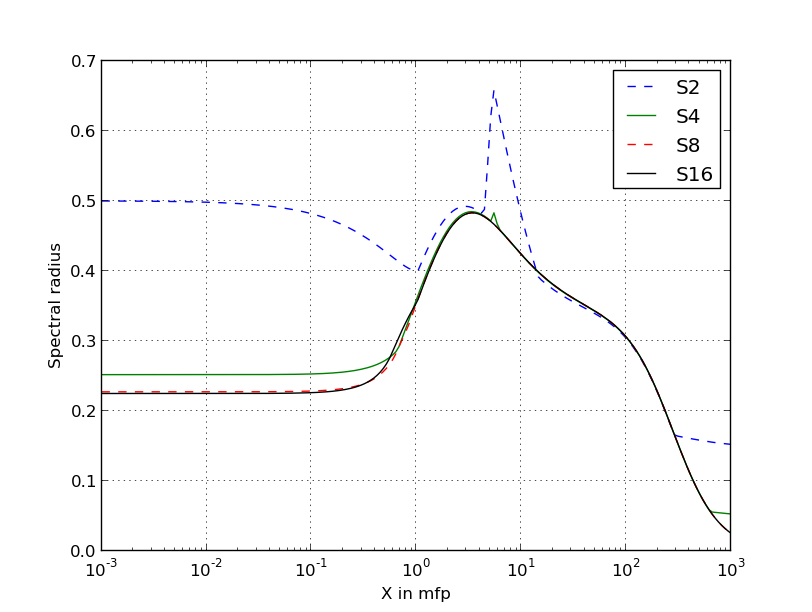
\includegraphics[width=0.5\textwidth]{sn_order_9999}
  \caption{Fourier analysis as a function of the mesh optical thickness,
  homogeneous infinite medium case}
  \label{fig_fa_sn}
\end{figure}
MIP is stable for every cell size. The spectral radius is always less than
0.5, except for $S_2$ where it is about 0.7.
\subsubsection{Aspect ratio varied}
For this Fourier analysis, we use a $S_{16}$ GLC quadrature, a homogeneous
medium, $c=0.9999$ and periodic boundary conditions. The $x-$axis is the mesh
size in mean free path in the $x$ direction and the $y-$axis is the spectral
radius. On \Cref{fig_fa_ar}, there are five curves corresponding to five
different aspect ratio: $\frac{Y}{X}=\frac{1}{16}$, $\frac{Y}{X}=\frac{1}{4}$,
$\frac{Y}{X}=1$, $\frac{Y}{X}=4$, $\frac{Y}{X}=16$, and $\frac{Y}{X}=100$.
\begin{figure}[H]
  \centering
  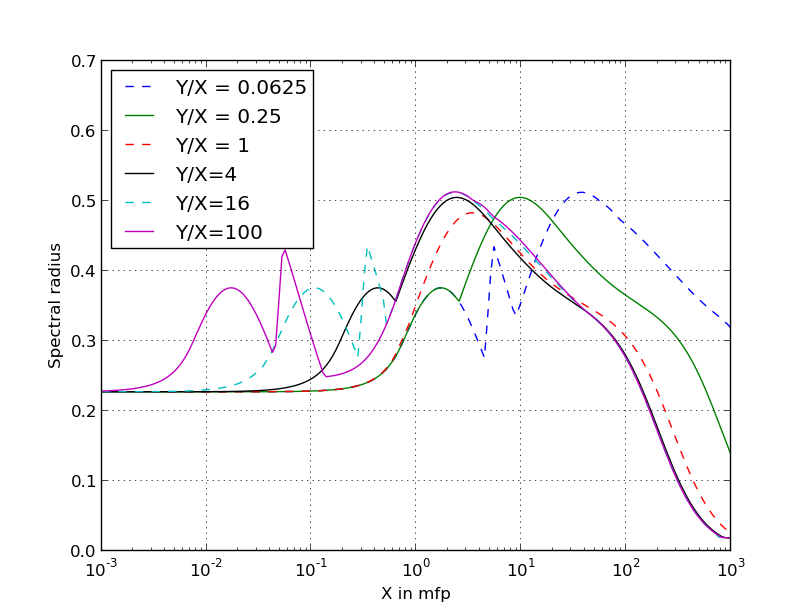
\includegraphics[width=0.5\textwidth]{aspect_ratio_9999_2}
  \caption{Fourier analysis as a function of the mesh optical thickness,
  homogeneous infinite medium case for different aspect ratios}
  \label{fig_fa_ar}
\end{figure}
MIP is stable for every the aspect ratio and the maximum of the spectral radius
is at about 0.5. When both $c$ approaches one and the aspect ratio is large,
MIP can become ill-conditioned.

\subsection{Homogeneous medium}
Next, we compare different solvers for MIP on a homogeneous medium, $100cm
\times 100cm$, $\Sigma_t = 1cm^{-1}$ and $\Sigma_s = 0.999cm^{-1}$, with
vacuum boundary conditions and a source of intensity $1cm^{-3}s^{-1}$. We
use a $S_8$ Gauss-Legendre-Chebyshev quadrature, a Source Iteration solver
with relative tolerance of $10^{-8}$ and a relative tolerance for MIP of
$10^{-10}$. The medium is discretized using two different meshes:
\begin{description}
  \item[Quadrilateral cells:] the mesh is composed of 49236 quadrilateral
    cells that to 197052 degrees of freedom.
  \item[Polygonal cells:] the mesh is composed of 45204 triangles, 823
    quadrilaterals, 4978 pentagons, 4155 hexagons, 725 heptagons, and 24
    octagons, for a total of 55909 cells and 193991 degrees of freedom. This
    example will allow us to test MIP and the different preconditioners on a
    mesh composed of different types of cell.
\end{description}
The meshes and the solutions of these problems are given on
\Cref{homog_test}:
\begin{figure}[H]
  \centering
  \begin{subfigure}{0.45\textwidth}
    \centering
    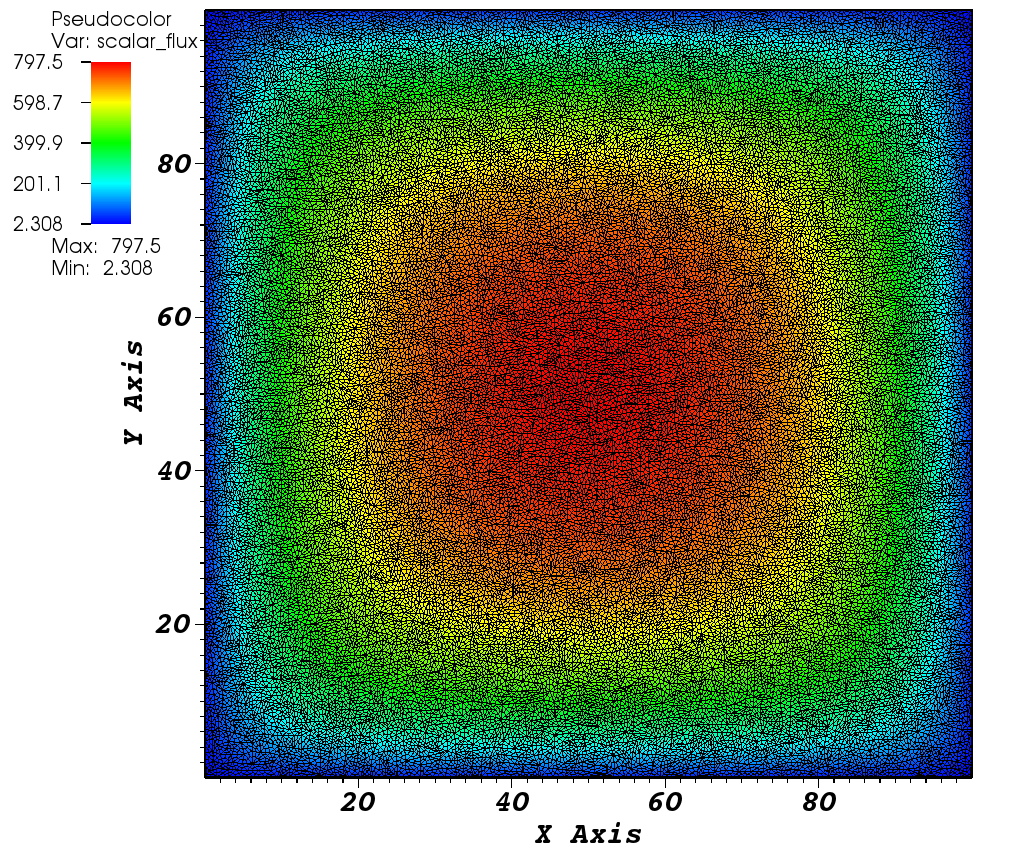
\includegraphics[width=\textwidth]{big_homog_quad_crop}
    \caption{Quadrilateral cells}
  \end{subfigure}
  \begin{subfigure}{0.45\textwidth}
    \centering
    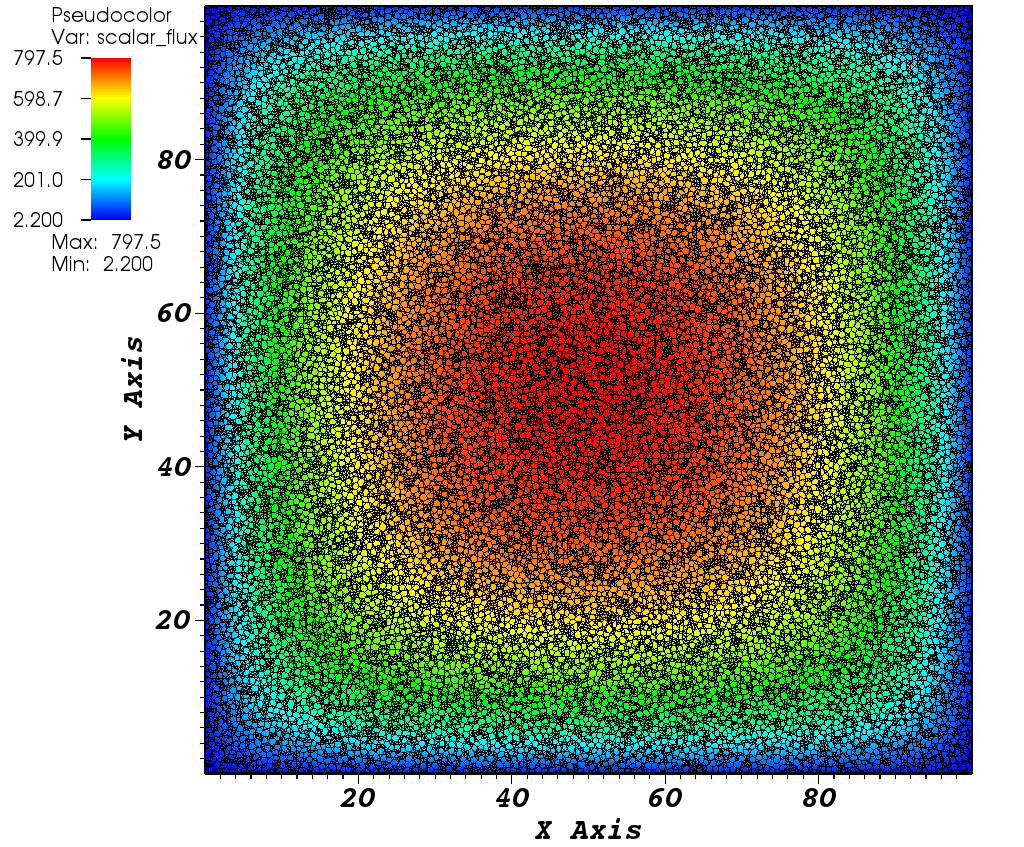
\includegraphics[width=\textwidth]{big_homog_poly_crop}
    \caption{Polygonal cells}
  \end{subfigure}
  \caption{Meshes and scalar fluxes}
  \label{homog_test}
\end{figure}
In \Cref{comparison_homog_quad}, the different solvers, used on the
quadrilateral cells, are compared:
\begin{table}[H]
  \begin{center}
    \caption{Comparison of different preconditioners for quadrilateral cells}
    \begin{tabular}{|c|c|c|c|c|c|c|}
      \hline
      & No-DSA & CG & PCG-SGS & PCG-ML-Uncoupled & PCG-ML-MIS & AGMG \\
      \hline
      SI iterations   & 7311    & 24      & 24       & 24      & 24      & 24 \\
   Precond init (s)   & NA      & NA      & 0.171358 & 1.8255  & 9.56078 & 0.332 \\
MIP calculation (s)   & NA      & 1095.7  & 1311.76  & 192.622 & 197.632 & 29.9727 \\
      CG iterations   & NA      & 56649   & 17332    & 630     & 604     & 578 \\
Total calculation (s) & 39176.7 & 1264.98 & 1477.95  & 363.202 & 367.841 &
      194.568 \\
      \hline
    \end{tabular}
    \label{comparison_homog_quad}
  \end{center}
\end{table}
In this Table, SI iterations is the number iteration of Source Iteration
needed to solve the problem, Precond init is the time in seconds needed to
initialize the preconditioner used by CG, MIP calculation is the total time in
seconds spent solving DSA during the calculation, CG iterations is the total number 
of CG iterations used to solve MIP, and Total calculation is the time in
seconds needed to solve the problem.

Using MIP decreases significantly the number of SI iterations and the
calculation time as expected. Using PCG-SGS decreases by a factor of three of
the number of CG iterations compared to CG but the time needed to solve MIP is
greater. This is because each PCG-SGS iteration is much slower than one
unpreconditioned CG iterations. The profiling of the code shows that the
bottleneck is the function 
\emph{Ifpack\_PointRelaxation::ApplyInverseSGS\_FastCrsMatrix} of Trilinos. This
function applies the forward and the backward substitutions required by SGS.
It is unclear why these substitutions are so costly. With ML, the number of CG
iterations is reduced by a factor of 50 and the MIP calculation time is
reduced by a factor three compared to CG. AGMG is by far the most efficient
solver, the number of CG iterations is slightly lower than PCG-ML but the MIP
calculation is 20 times faster than CG. The reason why there is such a big
difference between AGMG and PCG-ML is due to SGS. SGS is used as pre- and
post-smoother in ML and the function
\emph{Ifpack\_PointRelaxation::ApplyInverseSGS\_FastCrsMatrix} is once again the
bottleneck of the method.

The different solvers, used int the polygonal cells, are compared in
\Cref{comparison_homog_poly}:
\begin{table}[H]
  \begin{center}
    \caption{Comparison of different preconditioners for polygonal cells}
    \begin{tabular}{|c|c|c|c|c|c|c|}
      \hline
      & No-DSA & CG & PCG-SGS & PCG-ML-Uncoupled & PCG-ML-MIS & AGMG \\
      \hline
      SI iterations   & 7311    & 23      & 23      & 23      & 23      & 23 \\
   Precond init (s)   & NA      & NA      & 0.06388 & 1.73379 & 8.0426  & 0.388 \\
MIP calculation (s)   & NA      & 877.861 & 1263.31 & 198.63  & 191.989 &
      31.242 \\
      CG iterations   & NA      & 46262   & 16712   & 652     & 603     & 555 \\
Total calculation (s) & 42666.7 & 1060.53 & 1447.53 & 382.275 & 384.422 &
      216.946 \\
      \hline
    \end{tabular}
    \label{comparison_homog_poly}
  \end{center}
\end{table}
We see that using different types of cells in the same mesh does not affect
the performance of MIP or of the preconditioners.

\subsection{Heterogeneous medium}
In this example, we use a heterogeneous medium composed of 184 triangles, 3720
quadrilaterals and 2791 regular hexagons of side $0.05cm$ for a total of 6695 
cells and 32178 degrees of freedom. The domain is $5.28275cm$ by $4.6cm$. 
Reflective boundary conditions are used. The quadrature is a $S_{16}$ 
Gauss-Legendre-Chebyshev quadrature. The SI solver has a relative tolerance of 
$10^{-8}$ and the relative tolerance for MIP is $10^{-10}$. The domain is 
composed of three zones:
\begin{figure}[H]
\centering
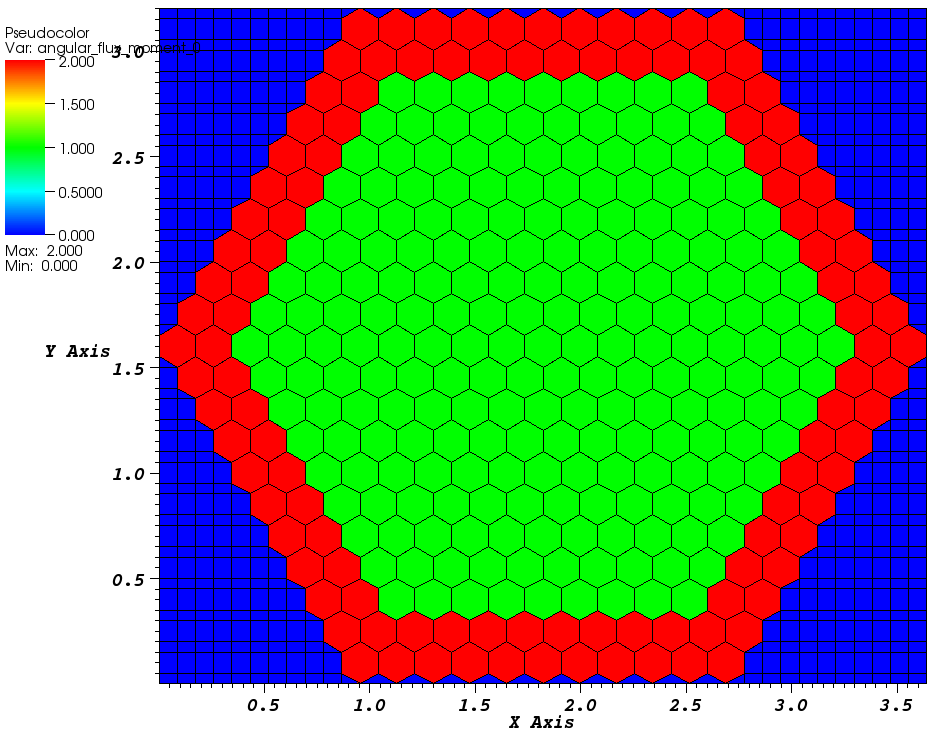
\includegraphics[width=0.4\textwidth]{source_crop}
\caption{Zones of the domain}
\end{figure}
The properties of the different zones are:
\begin{description}
\item[Green zone:] $\Sigma_t =1.5$cm$^{-1}$, $\Sigma_s = 1.499$cm$^{-1}$, source$ =
1$cm$^{-3}$s$^{-1}$
\item[Red zone:] $\Sigma_t = 1$cm$^{-1}$, $\Sigma_s = 0.999$cm$^{-1}$, no source
\item[Blue zone:] $\Sigma_t = 1$cm$^{-1}$, $\Sigma_s = 0.3$cm$^{-1}$, no source
\end{description}
The different solvers are compared in \Cref{comparison_hex}:
\begin{table}[H]
  \begin{center}
    \caption{Comparison of preconditioners with heterogeneous medium}
    \begin{tabular}{|c|c|c|c|c|c|c|}
      \hline
      & No-DSA & CG & PCG-SGS & PCG-ML-Uncoupled & PCG-ML-MIS & AGMG\\
      \hline
      SI iterations & 278     & 17      & 17        & 17       & 17      & 17  \\
   Precond init (s) & NA      & NA      & 0.0160661 & 0.368768 & 1.41632 &
      0.07  \\
MIP calculation (s) & NA      & 58.422  & 126.93    & 33.2225  & 31.3045 &
      2.924 \\
      CG iterations & NA      & 12214   & 6679      & 415      & 386     & 248  \\
Total calculation (s) & 910.566 & 120.889 & 190.413 & 99.7524  & 97.4666 &
      70.6424 \\      
      \hline
    \end{tabular}
    \label{comparison_hex}
  \end{center}
\end{table}
We can see that the comments that were done for the homogeneous tests are
still valid. MIP is effective even with heterogeneous medium and AGMG is
still the fastest solver. It is interesting to note that, contrary to the
homogeneous tests where the number of CG iterations remained similar for all
algebraic multigrid preconditioners, for this heterogeneous test AGMG requires
significantly fewer iterations than PCG-ML-Uncoupled and PCG-ML-MIS. This
difference may be due to the fact that ML was first designed to be used for
continuous finite elements discretization and that we are using discontinuous
finite elements.

\subsection{AMR mesh}
In this example \cite{mip}, the domain is $10cm\times 10cm$. The left and bottom
boundaries are reflective whereas the right and the top boundaries are vacuum. 
There are 10720 cells: 10482 quadrilaterals, 236 pentagons,
and 2 hexagons for a total of 43120 degrees of freedom. 
As in the previous example, the domain is composed if three zones (see
\Cref{zone_amr}):
\begin{figure}[H]
  \centering
  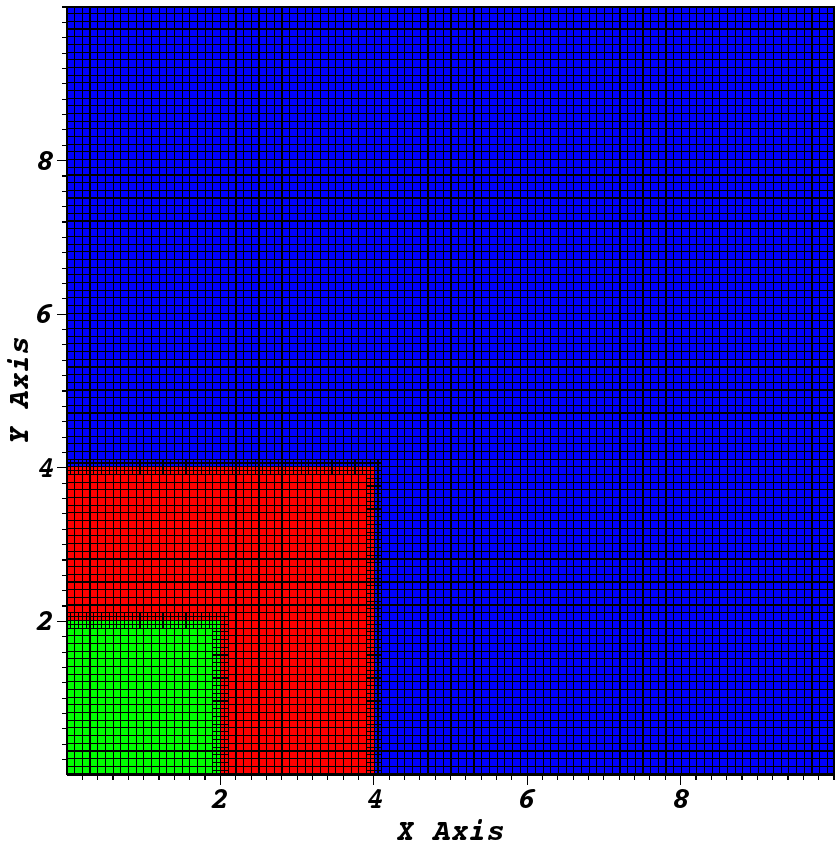
\includegraphics[width=6cm]{zone_amr}
  \caption{Polygons distribution}
  \label{zone_amr}
\end{figure}
where:
\begin{description}
  \item[Green zone:] $\Sigma_t=1.5cm^{-1}$, $\Sigma_s=1.44cm^{-1}$,
    source=$1cm^{-3}s^{-1}$
  \item[Red zone:] $\Sigma_t=1cm^{-1}$, $\Sigma_s=0.9cm^{-1}$, no source
  \item[Blue zone:] $\Sigma_t=1cm^{-1}$, $\Sigma_s=0.3cm^{-1}$, no source
\end{description}
The distribution of cells is given \Cref{fig_pol_dist} by:
\begin{figure}[H]
  \centering
  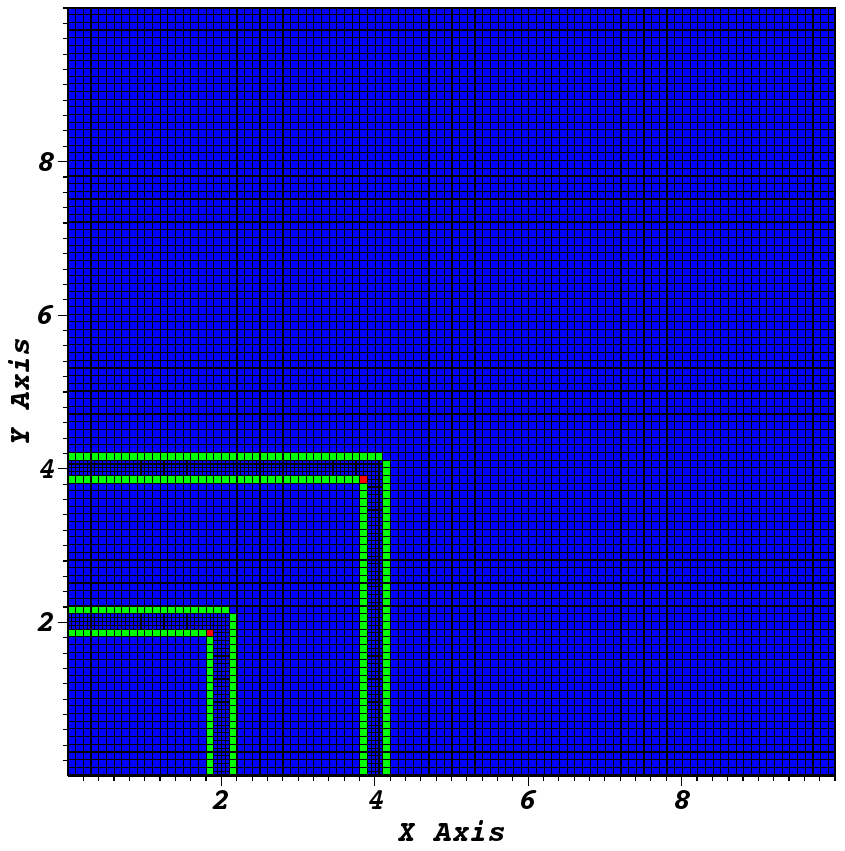
\includegraphics[width=6cm]{polygon_amr}
  \caption{Polygons distribution}
  \label{fig_pol_dist}
\end{figure}
where:
\begin{description}
  \item[Blue cells] are quadrilaterals.
  \item[Green cells] are pentagons.
  \item[Red cells] are hexagons.
\end{description}
This mesh is typical of a mesh obtained after one level of adaptive mesh
refinement (the cells at the interface of different zones have been refined
once). We see that instead of introducing hanging nodes, we have introduce
pentagons and hexagons in the mesh.
A $S_{16}$ GLC quadrature is employed. The tolerance on SI is $10^{-8}$ and
the tolerance on the CG solvers is $10^{-10}$.
The different solvers are compared in \Cref{table_amr}:
\begin{table}[H]
  \caption{Comparison of preconditioners on AMR mesh}
  \begin{center}
    \begin{tabular}{|c|c|c|c|c|c|c|}
      \hline
       & No-DSA & CG & PCG-SGS & PCG-ML-Uncoupled & PCG-ML-MIS & AGMG \\
      \hline
   SI iterations & 184     & 19      & 19       & 19      & 19       & 19 \\
Precond init (s) & NA      & NA      & 0.043463 & 0.358002 & 1.19301 & 0.0111\\
MIP calculation (s) & NA   & 48.1908 & 81.0992  & 25.2699 & 25.0699  & 
      2.56198\\
   CG iterations & NA      & 11300   & 4734     & 361     & 361      & 264 \\
     Total calculation (s) & 802.985 & 138.825 & 172.423  & 116.018 & 116.517  &
      94.1963\\
      \hline
    \end{tabular}
    \label{table_amr}
  \end{center}
\end{table}
As expected, the results are similar to our previous tests.

\subsection{Rectangular cells}
When the aspect ratio is high and the scattering ratio is close to one, MIP
becomes ill-conditioned. In the next two examples, the domain is square $100cm
\times 100cm$ with vacuum boundaries. There are 10000 cells and thus, 40000
degrees of freedom. The relative tolerance on SI is $10^{8}$ and the relative
tolerance on CG is $10^{-10}$. We use a $S_8$ GLC quadrature, $\Sigma_t =
1cm^{-1}$, and $\Sigma_s = 0.999cm^{-1}$. The source $1n/(cm^3s)$. In the
first test, the domain is discretized by 100 cells along $x$ and 100 cells
along $y$ (the aspect ratio is one). In the second test, the domain is
discretized by 1000 cells along $x$ and 10 cells along $y$ (the aspect ratio
is 100).
\begin{table}[H]
  \caption{Comparison of preconditioners on rectangular mesh with an aspect
  ratio of 1}
  \begin{center}
    \begin{tabular}{|c|c|c|c|c|c|c|}
      \hline
       & No-DSA & CG & PCG-SGS & PCG-ML-Uncoupled & PCG-ML-MIS & AGMG \\
      \hline
      SI iterations & 7311      & 21      & 21      & 21       & 21      & 21 \\
   Precond init (s) & NA        & NA      & 0.01422 & 0.051373 & 1.13144 &
      0.044 \\
MIP calculation (s) & NA        & 32.3825 & 73.8422 & 24.0707  & 25.0065 &
      1.7114 \\
      CG iterations & NA        & 8363    & 4853    & 376      & 375     &
      221\\
Total calculation (s) & 7356.96 & 56.8993 & 98.2609 & 50.1247  & 51.5396 &
      25.9306 \\
      \hline
    \end{tabular}
    \label{table_ar_1}
  \end{center}
\end{table}
\begin{table}[H]
  \caption{Comparison of preconditioners on rectangular mesh with an aspect
  ratio of 100}
  \begin{center}
    \begin{tabular}{|c|c|c|c|c|c|c|}
      \hline
       & No-DSA & CG & PCG-SGS & PCG-ML-Uncoupled & PCG-ML-MIS & AGMG \\
      \hline
      SI iterations & 7304    & 24      & 24        & 24       & 24      & 24 \\
   Precond init (s) & NA      & NA      & 0.0164239 & 0.362463 & 1.03128 & 0.052 \\
MIP calculation (s) & NA      & 372.227 & 742.902   & 941.06   & 922.258 &
      6.93176 \\
      CG iterations & NA      & 84802   & 43466     & 14180    & 13896   & 821 \\
Total calculation (s) & 9035.6 & 414.301 & 784.77   & 985.796  & 966.77  &
      44.7032 \\
      \hline
    \end{tabular}
    \label{table_ar_100}
  \end{center}
\end{table}                  
As predicted, inverting MIP requires a lot more CG iterations when the aspect
ratio increases. PCG-ML-Uncoupled and PCG-ML-MIS are much more affected by the
increase of the aspect ratio than the other methods. AGMG is the least
affected by the change of aspect ratio.
